\documentclass[border=12pt]{standalone}
\usepackage[utf8]{inputenc}
\usepackage[T1]{fontenc}
\usepackage{lmodern}
\usepackage{tikz}
\usetikzlibrary{positioning,shapes.geometric,arrows.meta}

\definecolor{mxNavy}{HTML}{12405E}
\definecolor{mxBlue}{HTML}{2A85BE}
\definecolor{mxTask}{HTML}{EEF7FC}
\definecolor{mxLaneA}{HTML}{F7FAFC}
\definecolor{mxLaneB}{HTML}{F2F8FC}

\tikzset{
  startev/.style={circle, draw=green!55!black, fill=green!12, thick, minimum size=6.5mm, inner sep=0pt},
  endev/.style={circle, draw=red!65!black, fill=red!12, ultra thick, minimum size=6.5mm, inner sep=0pt},
  task/.style={rectangle, draw=mxBlue, fill=mxTask, thick, rounded corners=3pt, text width=2.8cm, minimum height=1.15cm, align=center, font=\scriptsize\sffamily},
  gtw/.style={diamond, draw=orange!75!black, fill=yellow!15, thick, aspect=1.25, minimum size=7mm, inner sep=1pt, font=\tiny\sffamily\bfseries},
  datastore/.style={cylinder, shape border rotate=90, draw=mxNavy, fill=white, thick, minimum height=0.85cm, minimum width=1.4cm, align=center, font=\tiny\sffamily},
  flow/.style={-{Stealth[length=2.2mm]}, thick, color=mxNavy},
  msg/.style={-{Stealth[length=2.2mm]}, thick, dashed, color=mxBlue},
  lbl/.style={font=\tiny\sffamily\bfseries, text=mxNavy, fill=white, inner sep=1.5pt}
}

\begin{document}
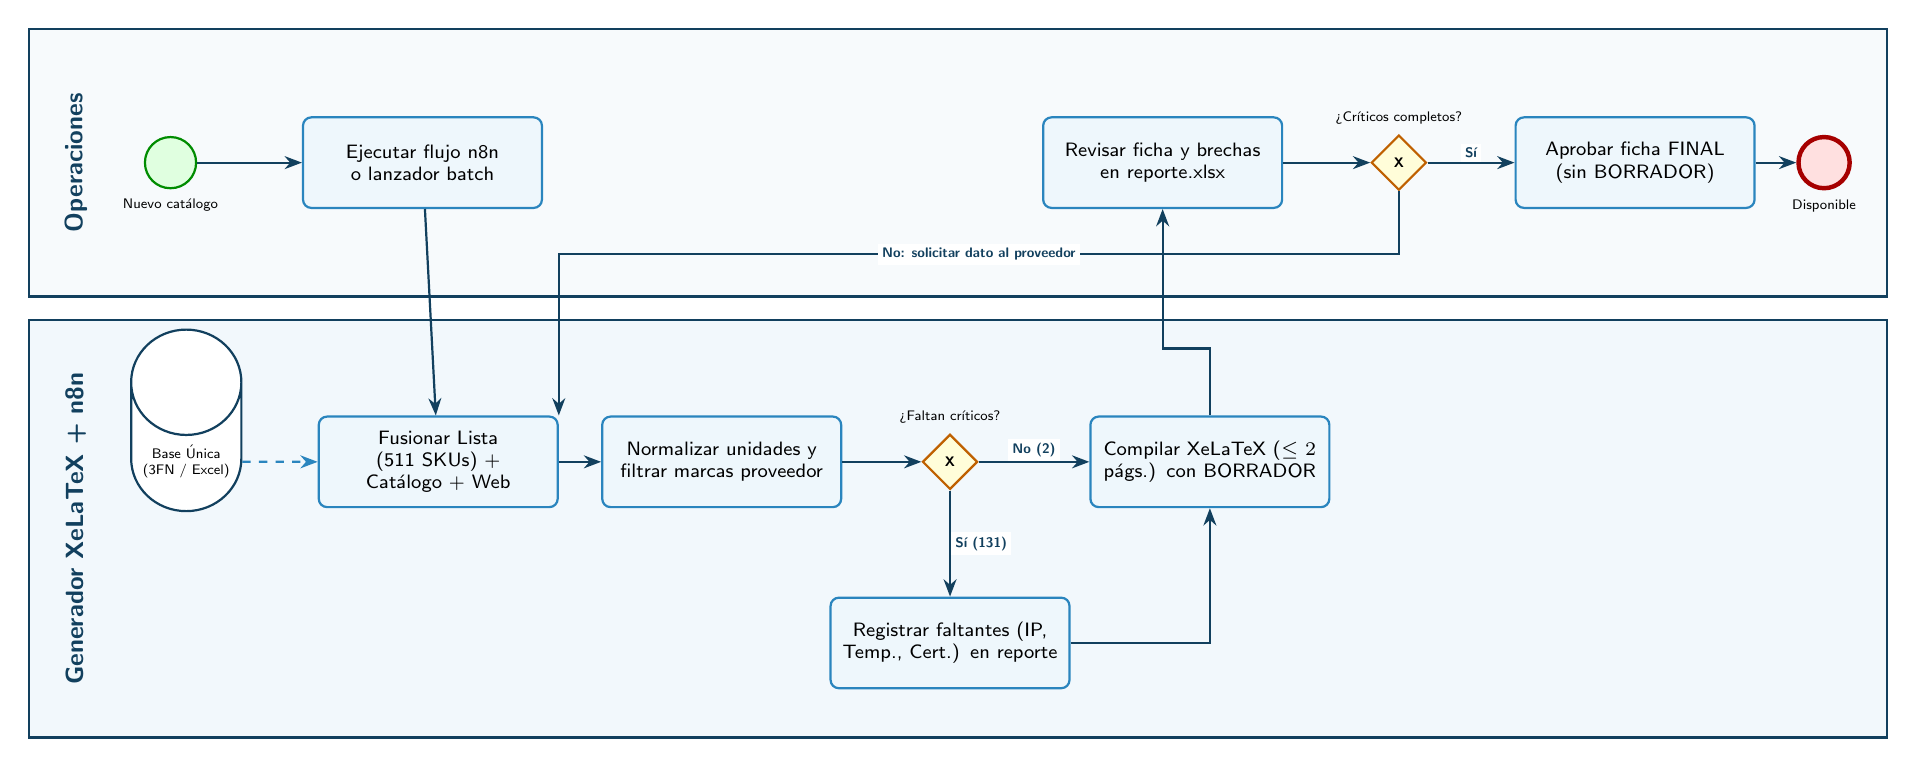
\begin{tikzpicture}

% --- CARRILES ALINEADOS ---
\draw[draw=mxNavy, fill=mxLaneA, thick] (-1.0, 5.2) rectangle (22.6, 8.6);
\node[font=\small\bfseries\sffamily, text=mxNavy, rotate=90] at (-0.4, 6.9) {Operaciones};

\draw[draw=mxNavy, fill=mxLaneB, thick] (-1.0, -0.4) rectangle (22.6, 4.9);
\node[font=\small\bfseries\sffamily, text=mxNavy, rotate=90] at (-0.4, 2.25) {Generador XeLaTeX + n8n};

% --- CARRIL SUPERIOR: OPERACIONES (y = 6.9) ---
\node[startev, label={[font=\tiny\sffamily]below:Nuevo catálogo}] (start) at (0.8, 6.9) {};
\node[task] (trig) at (4.0, 6.9) {Ejecutar flujo n8n o lanzador batch};
\node[task] (revisar) at (13.4, 6.9) {Revisar ficha y brechas en reporte.xlsx};
\node[gtw, label={[font=\tiny\sffamily]above:¿Críticos completos?}] (gok) at (16.4, 6.9) {X};
\node[task] (pub) at (19.4, 6.9) {Aprobar ficha FINAL (sin BORRADOR)};
\node[endev, label={[font=\tiny\sffamily]below:Disponible}] (fin) at (21.8, 6.9) {};

% --- CARRIL INFERIOR: GENERADOR (y = 3.1 y 0.8) ---
\node[datastore] (dsbase) at (1.0, 3.1) {Base Única\\(3FN / Excel)};
\node[task] (leer) at (4.2, 3.1) {Fusionar Lista (511 SKUs) + Catálogo + Web};
\node[task] (filt) at (7.8, 3.1) {Normalizar unidades y filtrar marcas proveedor};
\node[gtw, label={[font=\tiny\sffamily]above:¿Faltan críticos?}] (gcrit) at (10.7, 3.1) {X};
\node[task] (tex) at (14.0, 3.1) {Compilar XeLaTeX ($\le 2$ págs.) con BORRADOR};
\node[task] (pend) at (10.7, 0.8) {Registrar faltantes (IP, Temp., Cert.) en reporte};

% --- FLUJOS ---
\draw[flow] (start) -- (trig);
\draw[flow] (trig) -- (leer);
\draw[msg] (dsbase) -- (leer);
\draw[flow] (leer) -- (filt);
\draw[flow] (filt) -- (gcrit);
\draw[flow] (gcrit) -- node[lbl, above]{No (2)} (tex);
\draw[flow] (gcrit) -- node[lbl, right]{Sí (131)} (pend);
\draw[flow] (pend.east) -| (tex.south);
\draw[flow] (tex.north) -- ++(0,0.85) -| (revisar.south);
\draw[flow] (revisar) -- (gok);
\draw[flow] (gok) -- node[lbl, above]{Sí} (pub);
\draw[flow] (pub) -- (fin);
\draw[flow] (gok.south) -- ++(0,-0.8) -| node[lbl, pos=0.25]{No: solicitar dato al proveedor} (leer.north east);

\end{tikzpicture}
\end{document}
